
\section{Model comparison with measurements: anomalous heating in the edge.}\label{sec:results_results}
\begin{figure}
    \centering
    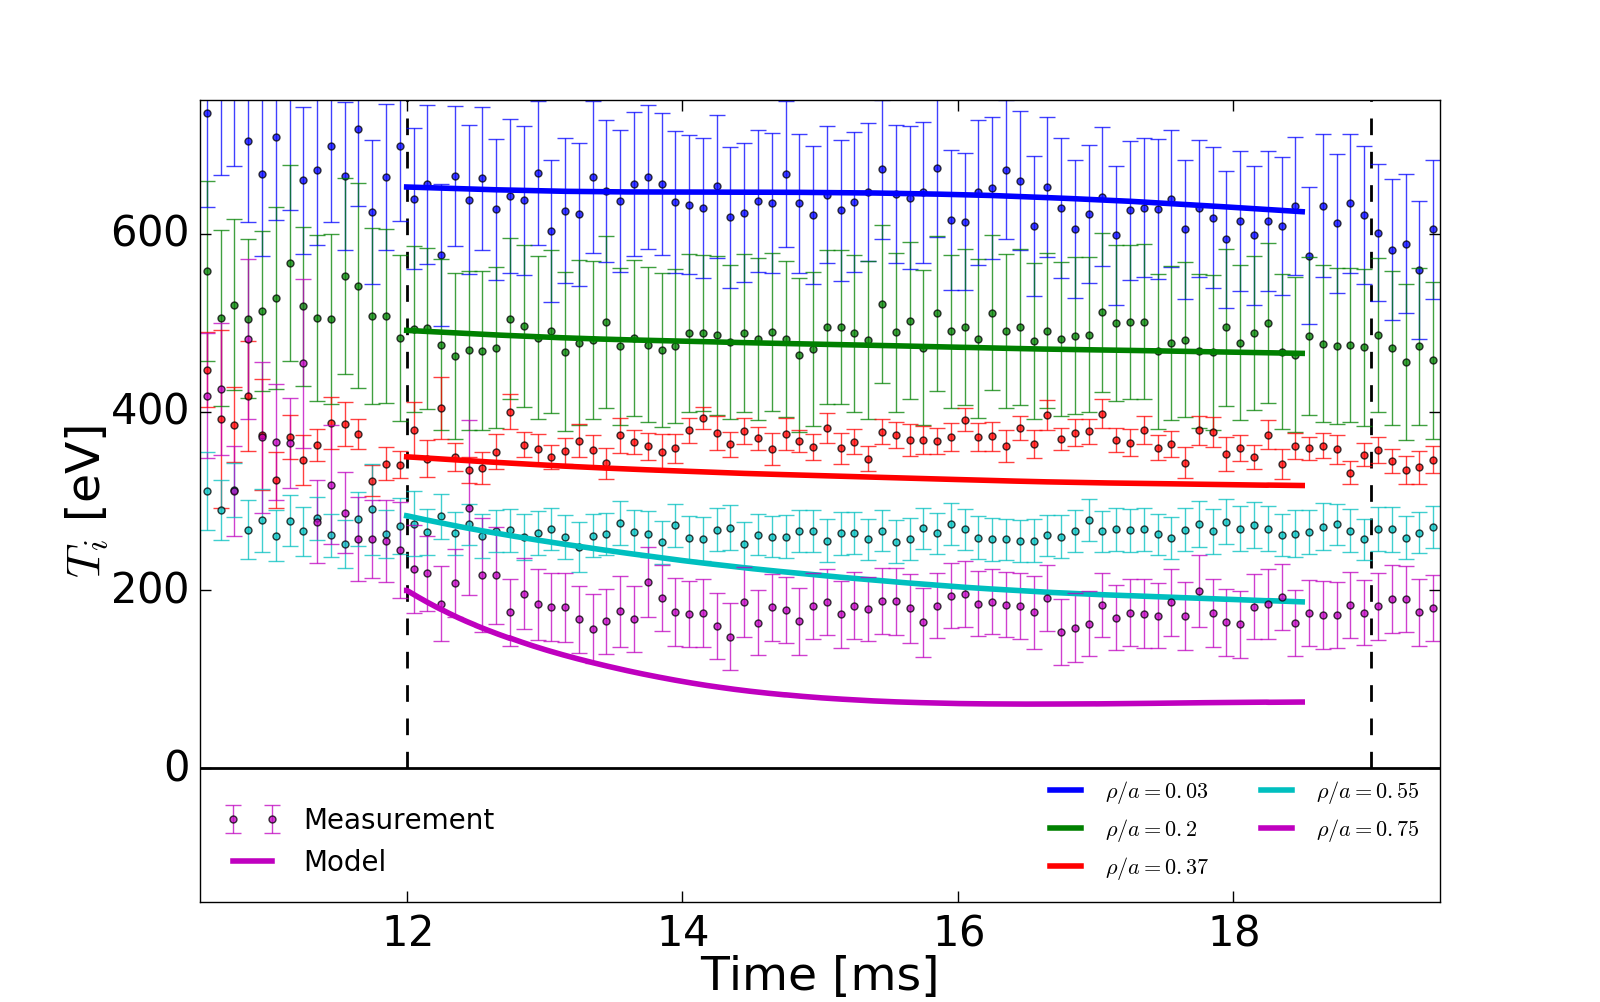
\includegraphics[width = \textwidth]{ion_transport_results/temperature_results.png}
    \caption[Temperature comparison with measurement]{Temperature comparison with measurement.}
    \label{fig:temperature_results}
\end{figure}

\begin{figure}
    \centering
    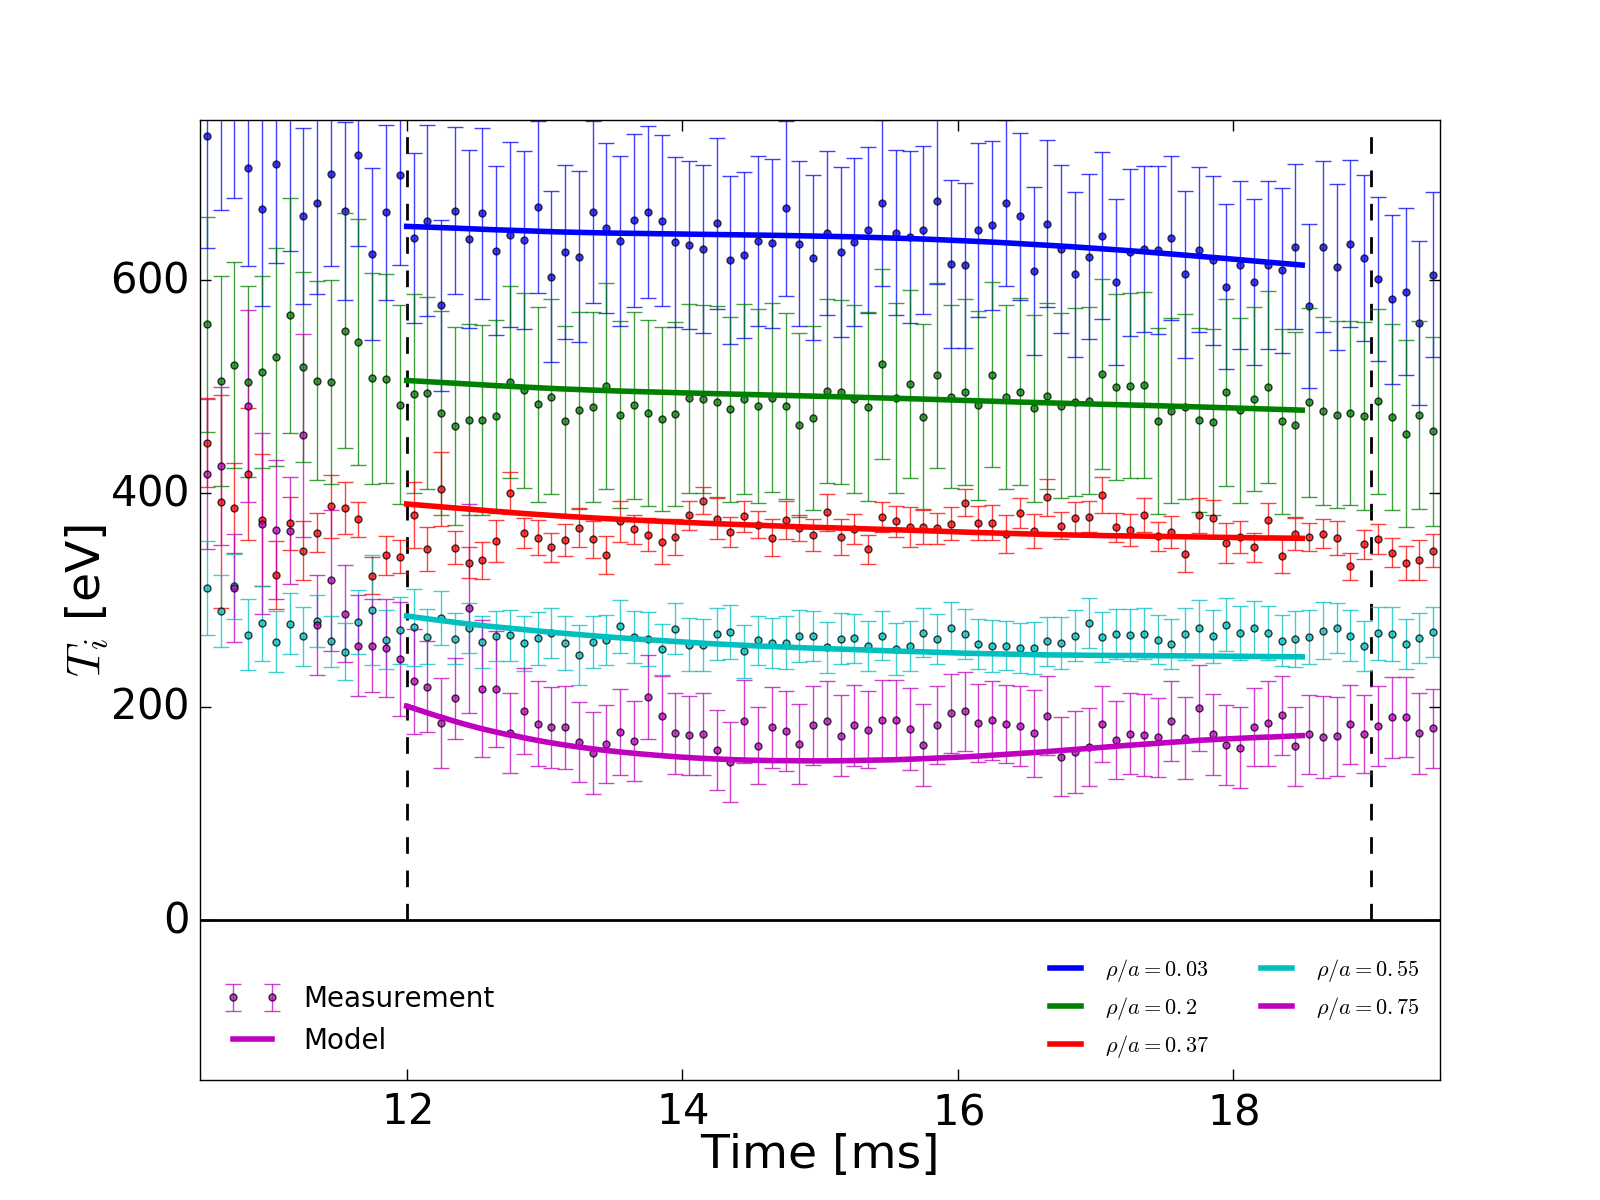
\includegraphics[width = \textwidth]{ion_transport_results/temperature_with_adhoc.png}
    \caption[Temperature comparison with measurement with \textit{ad hoc} term included]{Temperature comparison with measurement with \textit{ad hoc} term included.}
    \label{fig:temperature_results_ah}
\end{figure}

\begin{figure}
    \centering
    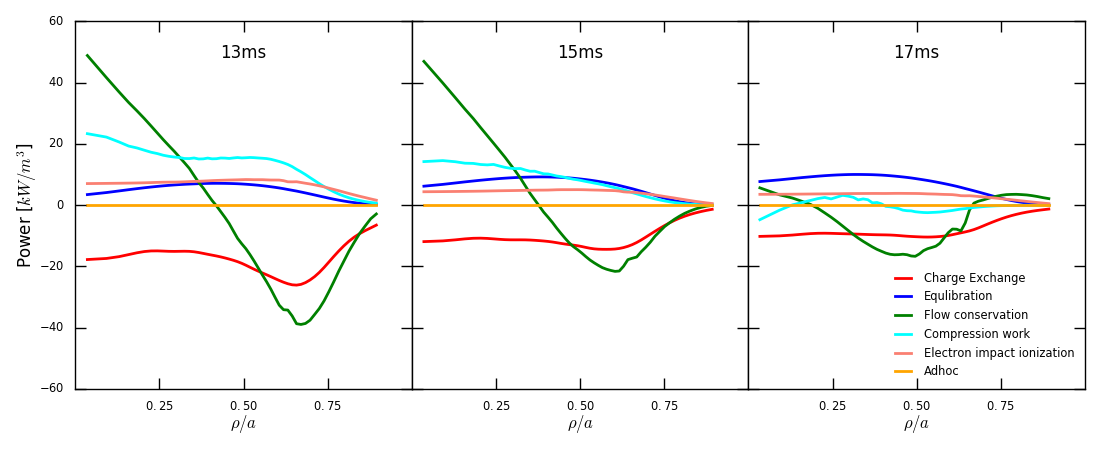
\includegraphics[width = \textwidth]{ion_transport_results/power_terms_no_adhoc.png}
    \caption[Power terms resulting from radial ion flow]{Power terms resulting from radial ion flow.}
    \label{fig:power_terms_no_ahoc}
\end{figure}
The quality of the model is evaluated by comparing its prediction to the ion temperature measurement made with CHERS. The model is initiated at 12ms, about 2ms after the first PPCD capacitor bank 'fires', as it is the earliest time when the significant suppression of tearing mode turbulence are achieved. CHERS measurement of temperature at initialization time is fit to an alpha model profile and then input into the model as initial condition. The time evolution of ion temperature is calculated according to the physics terms described in the previous sections and chapters. The model is found to adequately predict the temperature in the core, but not in the edge. To account for the edge temperature, an \textit{ad hoc} heating term is added. The model comparison results can been seen in figure \ref{fig:temperature_results}.  The most significant power loss terms (figure \ref{fig:power_terms_no_ahoc}) affecting this region is charge exchange, and thermal energy carried by particle flow (flow conservation). It is interesting to note that these loss terms are to a large extent a function of temperature as much if not more than as a function of temperature gradient. This dependence on $T_i$ is a factor that result in there being an 'equilibrium' temperature for the model. For the case where no \textit{ad hoc} heating is included, the ion temperature at near the edge would decrease until it levels off at significantly lower temperatures than the measured. In particular, figure \ref{fig:temperature_results} superficially suggest that (for the edge chord location) the temperature decreases rapidly early during the PPCD period. But initializing the model at later starting time would have the model reproduce the same behavior and settle at the same edge temperature, just now delayed. This indicates that it is not some particular circumstance relating to the early PPCD period that causes the model to under predict the temperature. But the model behaves in such a way that the edge temperature trends towards and `equilibrium' temperature determined by the power terms, which is significantly lower than the actual equilibrium temperature that the ion fluid comes to. To remedy this under prediction, an \textit{ad hoc} term is introduced into the model to raise the model's 'equilibrium'. The particular profile shape and location used for the \textit{ad hoc} term is discussed in detail in the next section, but the result of this are presented in figure \ref{fig:temperature_results} and \ref{fig:power_terms_with_adhoc}. With this addition, the model is able to account for the temperatures measured by CHERS. In this scenario, the core power terms are dominated by the effects of flow, in particular compressional heating and flow conservation. It is also useful to refer to figure \ref{fig:temperature_change} which provides information on how each term effects $T_i$. From this figure it is easier to see the importance of the compressional heating term on the core temperature prediction. $P_{\text{comp work}}$ is the larger of only two terms increasing temperature in the core, and is a major part of how the model matches a flat-ish fore $T_i$ evolution observed. Towards the edge, the major heating (thermal energy input) term is the \text{ad hoc} term. $P_{\text{flow cons}}$ is negative in the edge and the most significant source of loss. One looking at $\partialt T_i$ plot would come to the (almost) paradoxical conclusion the the flow conservation term is significant in maintaining temperature. This can be understood by pointing out the outward particle flow in the edge have the net effect of removing a number of ions at the local temperature, and replacing them with a smaller number of hotter ions from inner flux surfaces, thus increasing temperature. The density balance is achieved though a large ionization source rate, which reduces $T_i$ despite bringing some thermal energy with it (due to non-zero neutral temperature).


\begin{figure}
    \centering
    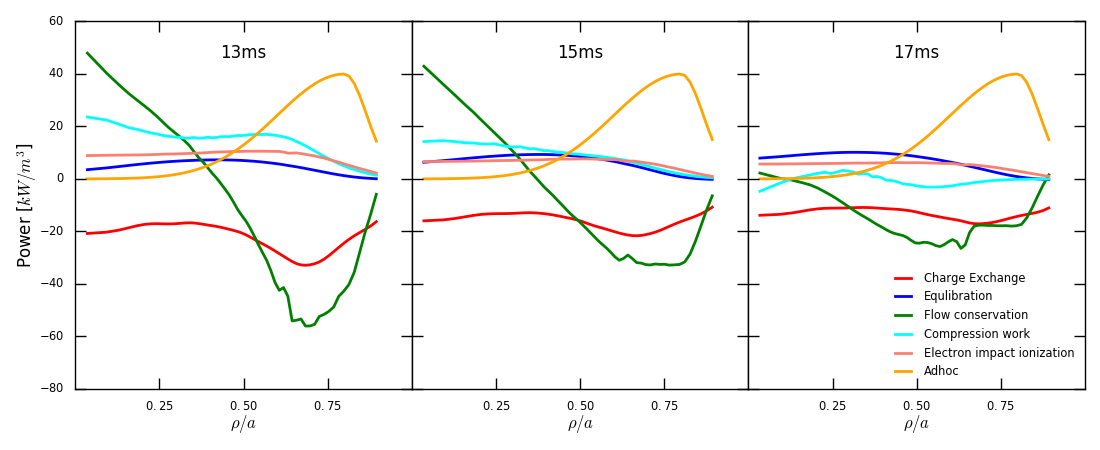
\includegraphics[width = \textwidth]{ion_transport_results/power_terms_with_adhoc.png}
    \caption[Power terms resulting from radial ion flow]{Power terms resulting from radial ion flow. Classical conduction have been omitted as it is of lower magnitudes than the plotted terms.}
    \label{fig:power_terms_with_adhoc}
\end{figure}


\begin{figure}
    \centering
    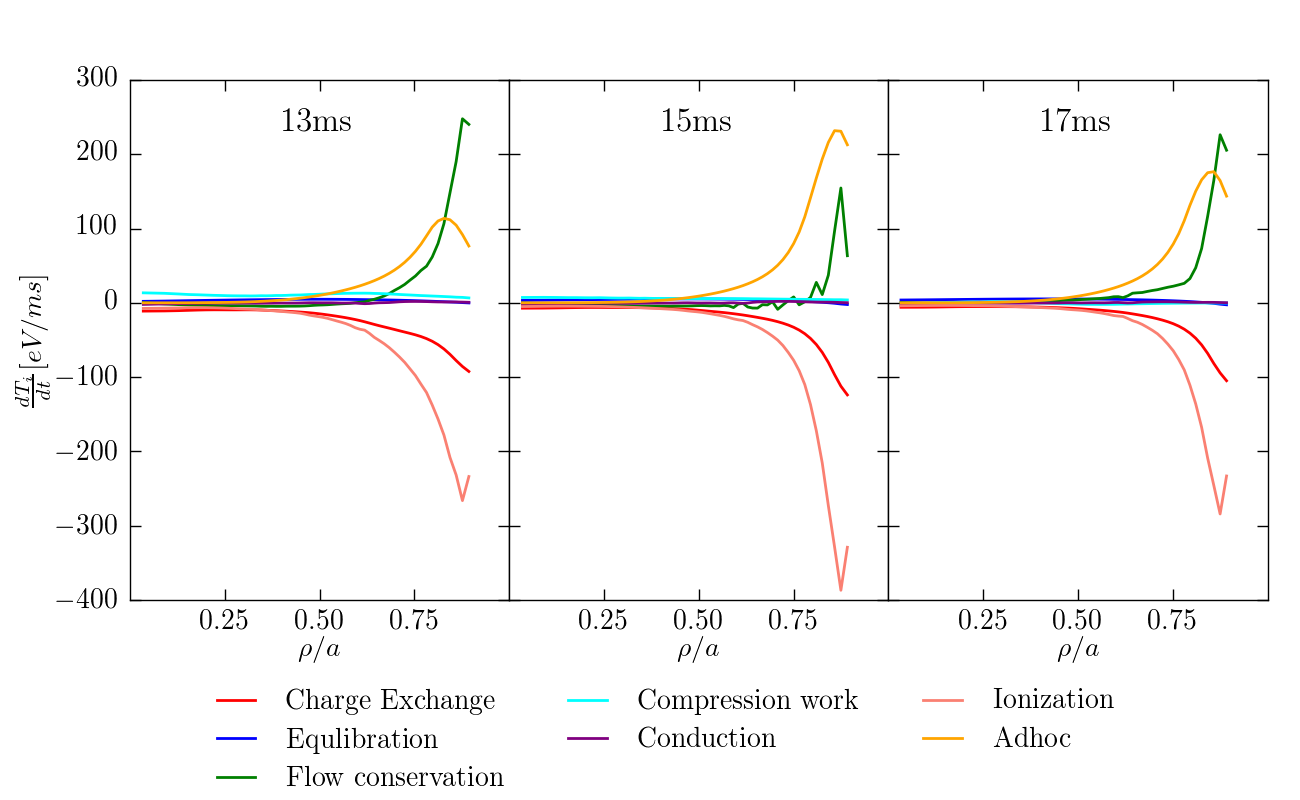
\includegraphics[width = 0.4\textwidth]{ion_transport_results/dtempdt_with_adhoc.png}
    \caption[$\partialt T_i$ due to various terms]{$\partialt T_i$ due to various terms in the model.}
    \label{fig:temperature_change}
\end{figure}

%TODO: There should be a paragraph on estimating the ion thermal confinement time that I'm not quite ready to write yet. 

From this model, the ion thermal confinement time can be estimated. The common definition of thermal confinement time is written as follows,
\begin{align}
    \tau_E &= \frac{W}{P_{\text{loss}}}
    &= \frac{W}{\partialt W - P_{\text{ohm}}}
\end{align}
However, in the context of the model, where the loss terms are known explicitly, it is more appropriate to specify $P_{\text{loss}}$ directly. In particular, 
\begin{align}
    P_{\text{loss}} &= - [P_{\text{CX}} + P_{\text{cond}} + P_{\text{flow cons}}]
\end{align}
The other terms in the model, including compressional work, \adhoc heating, and e-i equilibration heating, are considered 'external' power inputs, and thus do no factor into the calculation of the thermal confinement time. This means that for the consideration of this calculation, the flow terms as specified in section \ref{sec:flow_effects} are separated into the compressional heating part ($P_{\text{comp work}}$) which is not part of $P_{\text{loss}}$, and the flow conservation part ($P_{\text{flow cons}}$) which is. The confinement time of the model is shown in figure \ref{fig:conf_time}. It should be noted that this is not a direct measurement of the ion confinement time, but rather it is the ion confinement of a model that can matched observed temperature evolution.
\begin{figure}
    \centering
    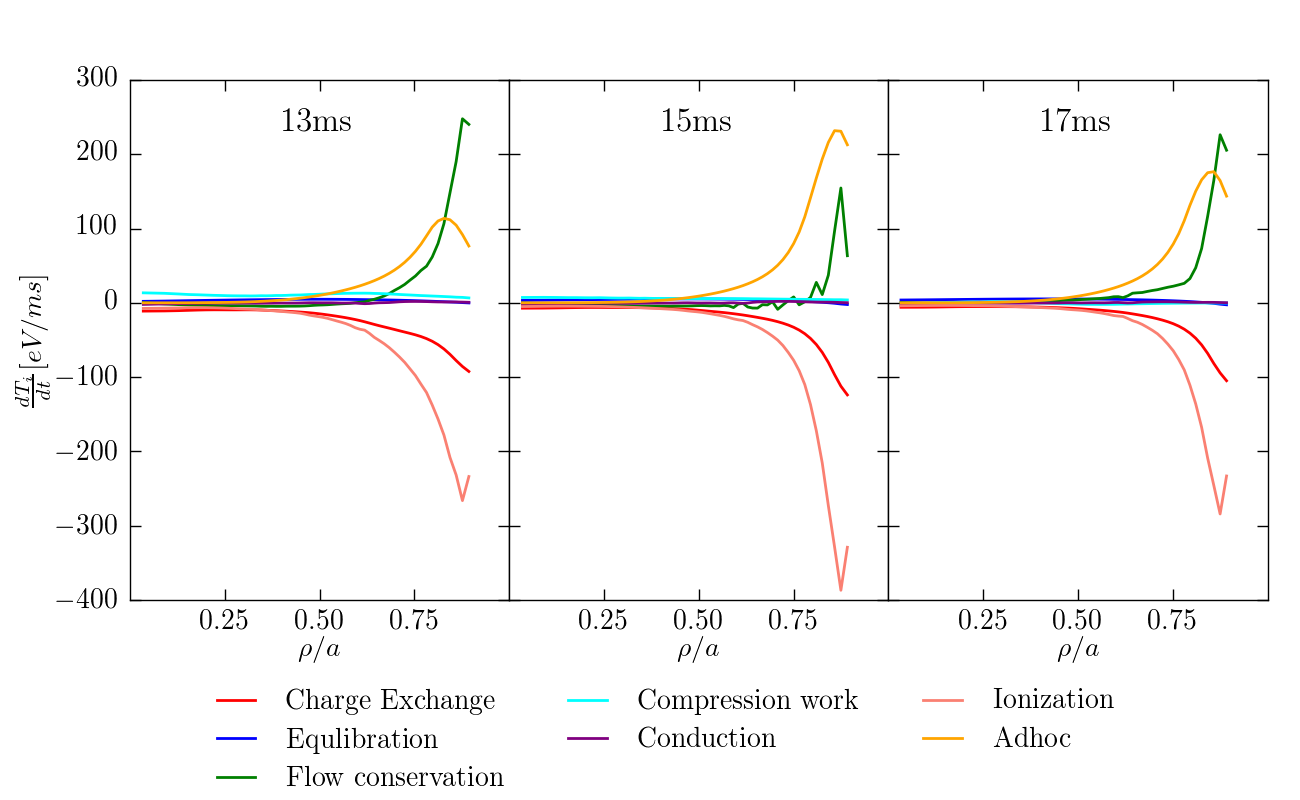
\includegraphics[width = 0.8\textwidth]{ion_transport_results/dtempdt_with_adhoc.png}
    \caption[Confinement time]{Estimated ion confinement time.}
    \label{fig:conf_time}
\end{figure}



\subsection{Profile and extent of \adhoc heating in the gradient regions}\label{sec:anomalous_heating}

The previous section glossed over the shape and location of the \textit{ad hoc} heating term used in order to present the results. However, there are comments to be made that would be of interest to readers. The driving determinant of the \textit{ad hoc} term is to enable the model to match the observations, but that does not mean that it is entirely free of physics considerations. The profile settled upon is an asymmetrical Gaussian (in $\rho_v$) made from two half Gaussian profiles with differing width. The profile peaks at $\rho_v/a = 0.75$, the approximate location of the reversal surface (see figure \ref{fig:q_profile}). The reversal surface is not only the home of all m = 0 modes, but also near tightly packed m =1 rational surfaces. Additionally, the peak and the width of the \textit{ad hoc} heating term is approximately coincident with the $T_e$ gradient region as measured via Thomson scattering. The edge half of the Gaussian shape have a smaller width to account for the fact that the turbulence that likely drives anomalous heating would be rapidly decreasing near MST's conducting shell, together with rapidly decreasing availability of free energy as temperature and density drops in the very edge. However, the modeling work and the CHERS measurements provide nearly no constraint on the very edge of the plasma. 

One of the candidate to explain anomalous ion heating in MST is the stochastic heating mechanism set out by G. Fiksel\cite{Fiksel2009}. The stochastic ion heating process produces a heating rate of:
\begin{align}
    a =b+c\\
    \text{TODO: find the actual equation}
\end{align}
The work of T. Nishizawa\cite{Nishizawa2018} measured the drift wave turbulence in the plasma edge in high current PPCD (400kA, so not quite an identical case, but it makes an instructive comparison). Using these information to estimate the heating from stochasticity

More generally, the location and the width of the \textit{ad hoc} heating term roughly corresponds with the location of the $T_e$ and $n_e$ gradient regions (see figure \ref{fig:ad_hoc_v_gradient}. While electron gradients are not directly connected to ion thermal heating, they are sources of free energy driving turbulence that would generate heating. 

\begin{figure}
    \centering
    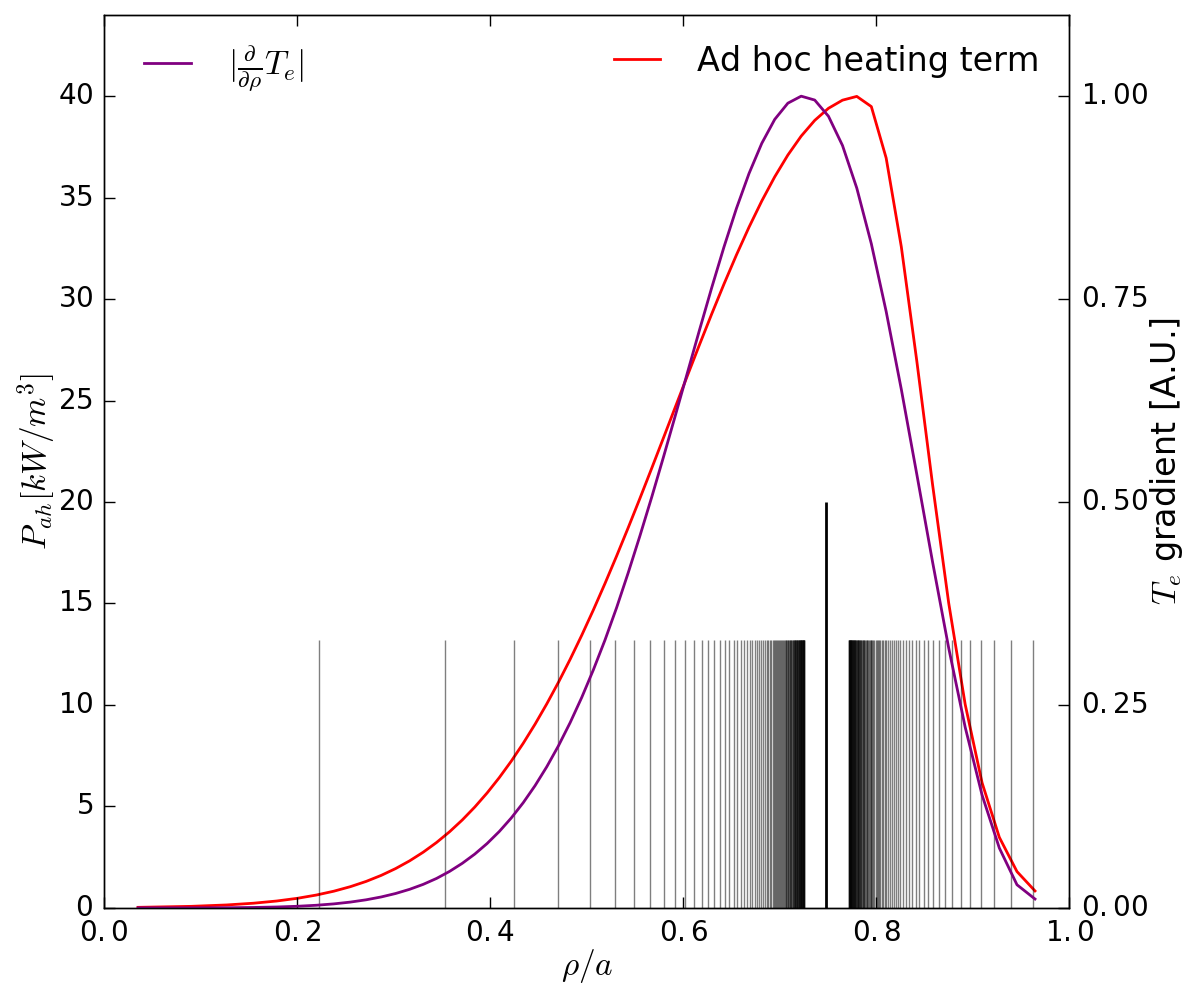
\includegraphics[width = 0.9\textwidth]{ion_transport_results/adhoc_profile.png}
    \caption[\textit{ad hoc} heating profile compared to gradients]{\textit{ad hoc} heating profile compared to normalized $T_e$ and $n_e$ gradients.}
    \label{fig:ad_hoc_v_gradient}
    %% Consider including the edge stochastic heating estimate.
\end{figure}

\subsection{Anomalous Transport vs. heating}

The \textit{ad hoc} heating term needed for the model can correspond to anomalous transport or heating, as the model does not account for stochastic transport mechanisms, or turbulent heating mechanisms. However, given the model's ability to predict the core temperature well even in the absence of the \textit{ad hoc} term, it is more likely that the discrepancy in the edge is accounted for by anomalous heating. 
Consider stochastic transport of heat, the stochastic counterpart to classical thermal conduction. The stochasticity increases the characteristic step size of the particle beyond the gyro-radius, and ions wondering along the stochastic field would collide another and exchange place' with it, transporting heat from the hotter location to the colder. Note that this is a purpose effort to separate the stochastic heat conduction/transport from the stochastic particle transport, as the particle transport and flux is indirectly included in the model (see the discussion in section \ref{sec:stochastic_effects}). The total \adhoc term needed in the model integrates to about 140kW over the volume of the plasma. If the \adhoc term is 'caused' by a anomalous transport mechanism, then the transport mechanism would be taking the thermal energy from hotter regions (\textit{ie.} core). For an estimation, one can assume that such a transport mechanism takes heat from the core region defined by $\rho/a \leq 0.4$ and deposit at $0.4 \leq \rho/a \leq 0.9$ (refer to figure \ref{fig:ad_hoc_v_gradient}). Thus defined, the core region have a volume of $\approx 1.25 m^2$, and lose heat at $~110kW/m^2$ making it the most significant term in the core. Further assuming a nominal core density of $0.7 \times 10^{19}/m^3$, the core cooling implied by such a transport would be $\approx 100eV/ms$ in addition to what the model currently predicts. This is significantly larger core cooling than the observations would allow (refer to figure \ref{fig:temperature_results_ah}).

While it cannot be ruled out that the \adhoc term in the model is the result of a combination of a anomalous transport mechanism, and a (relatively) radially uniform anomalous heating mechanism, it is very unlikely to be the effect of a anomalous transport mechanism only. To the first order, the result point to an anomalous heating mechanism active in the $T_e$ gradient region.

\subsection{Additional comments on thermal transport}


Further reduction of the neutral content in PPCD would be beneficial. One of the benefits of PPCD is a significantly reduced charge exchange loss term, due to reduced wall interactions. 


Gradient in the far edge is difficult to sustain, as the particle flux is large and brings hot ions to the edge of the plasma. Combined with anomalous heating in the edge and thus wall boundary may be hotter than expected. 

While e-i equilibration is generally insufficient in sustaining high ion temperature at typical MST densities, resulting in the temperature discrepancy seen in PPCD plasmas. Extrapolating to typical tokamak densities, however, would imply that the equilibration heating would in crease by ~ 2 order of magnitude (both $n_e$ and $n_i$ would increase by an order of magnitude) while the biggest core loss term, charge exchange, would increase less as the neutral sourcing will increase will plasma density, but the neutral penetration will decrease correspondingly. 

But core ion heating will likely stay put, as the studies of crash heating PPCDs demonstrates.


%TODO: I both feel like there are more bits and peices to comment on, but nothing is coming to mind at this moment. I'm conflicted about if I want to save stuff for the last chapter, or should I just have the equivalent of discussions here. 
